\chapter{Thực nghiệm và đánh giá}
\label{chap:evaluation}
\section{Thiết lập thực nghiệm}
\subsection{Hai phép thăm dò cơ chế}
Để kiểm chứng hai giả thuyết H1 và H2, chúng tôi sử dụng Attention Mixing Probe, một phiên bản Decoder Qwen2.5 cho phép cung cấp trực tiếp tài liệu và hệ số trộn chú ý \(d\). Việc sử dụng tài liệu có sẵn giúp khảo sát riêng tác động của Attention Mixing, không phụ thuộc vào Decision Head hoặc quá trình truy hồi tự hồi quy.

Dữ liệu thí nghiệm được xây dựng từ các tập xác thực MuSiQue với câu hỏi yêu cầu 2, 3 và 4 bước suy luận. Dựa trên nhãn đoạn hỗ trợ của bộ dữ liệu, mỗi mẫu được cung cấp ba đoạn văn theo bốn cấu hình: 0:3, 1:2, 2:1 và 3:0, tương ứng với số đoạn hỗ trợ và đoạn gây nhiễu. Các đoạn được lấy mẫu một lần cho mỗi câu hỏi với seed 42 và được giữ cố định khi thay đổi hệ số trộn. Cả hai phép thăm dò đều khảo sát 33 giá trị \(d=i/32\), với \(i=0,\ldots,32\).

Đối với H1, mô hình được chạy ở chế độ suy luận để đo LM Loss trên các token đích tại từng giá trị \(d\). Đối với H2, các tham số mô hình được đóng băng và gradient của LM Loss theo hệ số \(d\) được ghi nhận thông qua hook, không thực hiện cập nhật tham số (learning rate bằng 0). Kết quả được tổng hợp trên 1.024 mẫu đối với các cấu hình 0:3, 1:2 và 2:1; riêng cấu hình 3:0 có 494 mẫu do điều kiện 2 bước không đủ ba đoạn hỗ trợ. Vì vậy, khi so sánh kết quả giữa các cấu hình, cần lưu ý sự khác biệt về thành phần mẫu và lượng thông tin hỗ trợ được cung cấp.

\subsection{Đối chứng hệ thống}
Để đánh giá hiệu quả của hệ thống ART, chúng tôi tiến hành thực nghiệm trên ba bộ dữ liệu MuSiQue, HotpotQA và 2WikiMultiHopQA, mỗi bộ gồm 500 mẫu. Ba phương pháp được đánh giá trên cùng tập câu hỏi và đáp án tham chiếu nhằm bảo đảm tính nhất quán trong quá trình so sánh.

Các phương pháp đối chứng bao gồm:

\begin{itemize}
\item \textbf{No-RAG:} Mô hình sinh câu trả lời trực tiếp từ câu hỏi mà không sử dụng tài liệu truy hồi.
\item \textbf{Vanilla RAG:} Mô hình truy hồi một lần dựa trên câu hỏi ban đầu, sử dụng 5 đoạn văn liên quan để hỗ trợ sinh câu trả lời.
\item \textbf{ART:} Hệ thống quyết định thời điểm truy hồi trong quá trình sinh, với 5 đoạn văn được lấy ở mỗi lượt truy hồi.
\end{itemize}
Cả ba phương pháp đều sử dụng kiến trúc nền Qwen2.5-3B-Instruct. Tuy nhiên, No-RAG và Vanilla RAG sử dụng checkpoint gốc, trong khi ART sử dụng checkpoint đã fine-tune. Vì vậy, kết quả so sánh phản ánh hiệu quả tổng thể của hệ thống ART, bao gồm cả quá trình fine-tuning và cơ chế truy hồi thích nghi, thay vì chỉ đo lường riêng tác động của việc lựa chọn thời điểm truy hồi.

Hiệu quả trả lời câu hỏi được đánh giá thông qua ba chỉ số Accuracy (Acc), Exact Match (EM) và token-level F1, sử dụng quy tắc chuẩn hóa và so khớp đáp án theo bộ đánh giá R-Search. Kết quả được tính trung bình trên toàn bộ mẫu và biểu diễn dưới dạng phần trăm.

Trong evaluator, Acc đo tỷ lệ dự đoán chứa ít nhất một đáp án tham chiếu dưới dạng chuỗi con, không phân biệt hoa thường. EM và F1 so khớp sau chuẩn hóa. Các quy tắc này khớp với mã đánh giá R-Search\cite{rsearch}.

\section{Kết quả}
\subsection{Kiểm chứng H1 và H2}
\textbf{H1.} \Cref{fig:h1} cho thấy LM Loss thay đổi theo hệ số trộn \(d\) và tỷ lệ tài liệu hỗ trợ so với tài liệu gây nhiễu. Khi cả ba tài liệu đều gây nhiễu (0:3), tăng \(d\) ban đầu chỉ làm LM Loss giảm nhẹ từ 1.3160 tại \(d=0\) xuống 1.2753 tại \(d=0.25\). Sau đó, LM Loss tăng lên 1.3943 tại \(d=1\). Khi có tài liệu hỗ trợ, LM Loss giảm rõ hơn. Các giá trị thấp nhất quan sát được với tỷ lệ 1:2, 2:1 và 3:0 lần lượt là 1.1295, 0.9495 và 0.8830, tại \(d\) xấp xỉ 0.656, 0.719 và 0.750.

Hiệu quả của Attention Mixing phụ thuộc vào thành phần bằng chứng. Tài liệu hỗ trợ có thể giúp giảm LM Loss, trong khi tài liệu gây nhiễu hạn chế lợi ích đó. Cả bốn đường đều tăng trở lại khi \(d\) tiến đến 1, cho thấy sử dụng tối đa thông tin truy hồi không nhất thiết có lợi nhất trong thí nghiệm. LM Loss được đo dưới teacher forcing nên chưa trực tiếp cho biết chất lượng câu trả lời khi mô hình sinh tự do. Ngoài ra, điều kiện 3:0 thiếu dữ liệu hai bước, nên cần thận trọng khi so sánh với các nhóm còn lại.
\begin{figure}[htbp]\centering
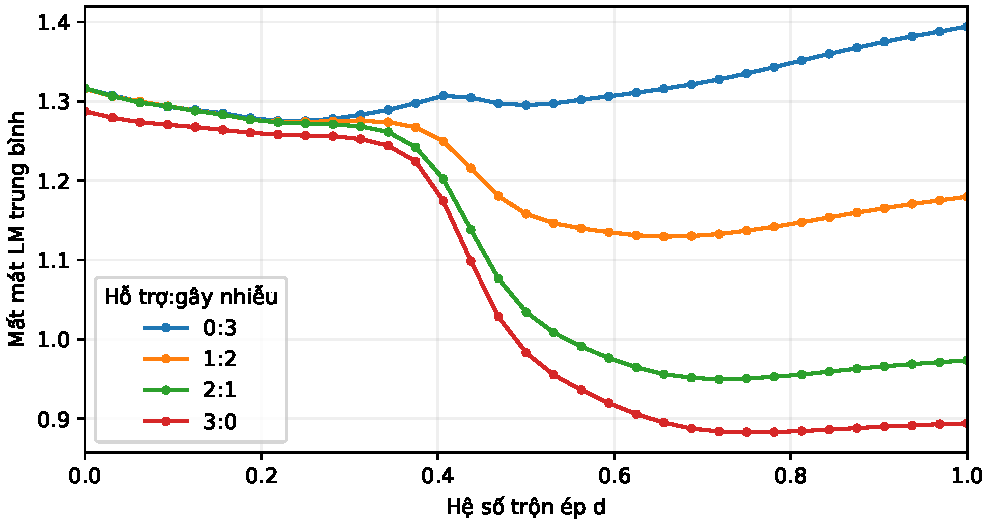
\includegraphics[width=.86\linewidth]{graphics/h1.pdf}
\caption{H1: mất mát trung bình trên đích theo hệ số trộn ép và tỷ lệ hỗ trợ:gây nhiễu. Nguồn: tổng hợp H1 của đề tài.}
\label{fig:h1}
\end{figure}

\pagebreak[4]
\textbf{H2.} \Cref{fig:h2,fig:h2cost} khảo sát gradient của LM Loss theo hệ số trộn \(d\). Gradient âm cho biết tăng nhẹ \(d\) có xu hướng làm giảm LM Loss tại điểm đang xét. Gradient dương cho biết tăng nhẹ \(d\) có xu hướng làm tăng LM Loss. Như vậy, độ dốc cung cấp tín hiệu cục bộ để mô hình học cách điều chỉnh mức sử dụng thông tin truy hồi.

Điều kiện chỉ chứa tài liệu gây nhiễu (0:3) có gradient dương lớn nhất tại \(d=0.375\), còn ba điều kiện có tài liệu hỗ trợ đạt gradient âm nhỏ nhất tại \(d=0.4375\). Sự khác biệt này gợi ý khảo sát vùng \(d\) khoảng 0.40--0.44, nơi tín hiệu gradient có thể phản ánh sự khác nhau giữa bằng chứng hỗ trợ và bằng chứng gây nhiễu. Gradient thay đổi theo \(d\), và tại \(d=1\) cả bốn điều kiện đều có gradient dương. Do đó, kết quả chưa cho thấy một giá trị \(d\) cố định phù hợp với mọi trường hợp.

Để khảo sát ảnh hưởng của chi phí truy hồi, \cref{fig:h2cost} minh họa điều kiện \(g(d)+\lambda=0\) qua các đường tham chiếu \(-\lambda\), với \(\lambda\) lần lượt bằng \(0\), \(0.05\) và \(0.1\). Các giao điểm cho biết những vị trí mà độ dốc của hàm mục tiêu có thể đổi dấu trong miền khảo sát. Chúng không xác định trực tiếp ngưỡng truy hồi tối ưu.

Trong thí nghiệm H1--H2, \(d\) là hệ số trộn được đặt trước. Khi mô hình sinh tự do, \(d_t\) là đầu ra của Decision Head. ART dùng ngưỡng vận hành \(\tau=0.4297\) theo kinh nghiệm để so sánh với \(d_t\). Các đồ thị H1--H2 không chứng minh đây là ngưỡng tối ưu.
\begin{figure}[htbp]\centering
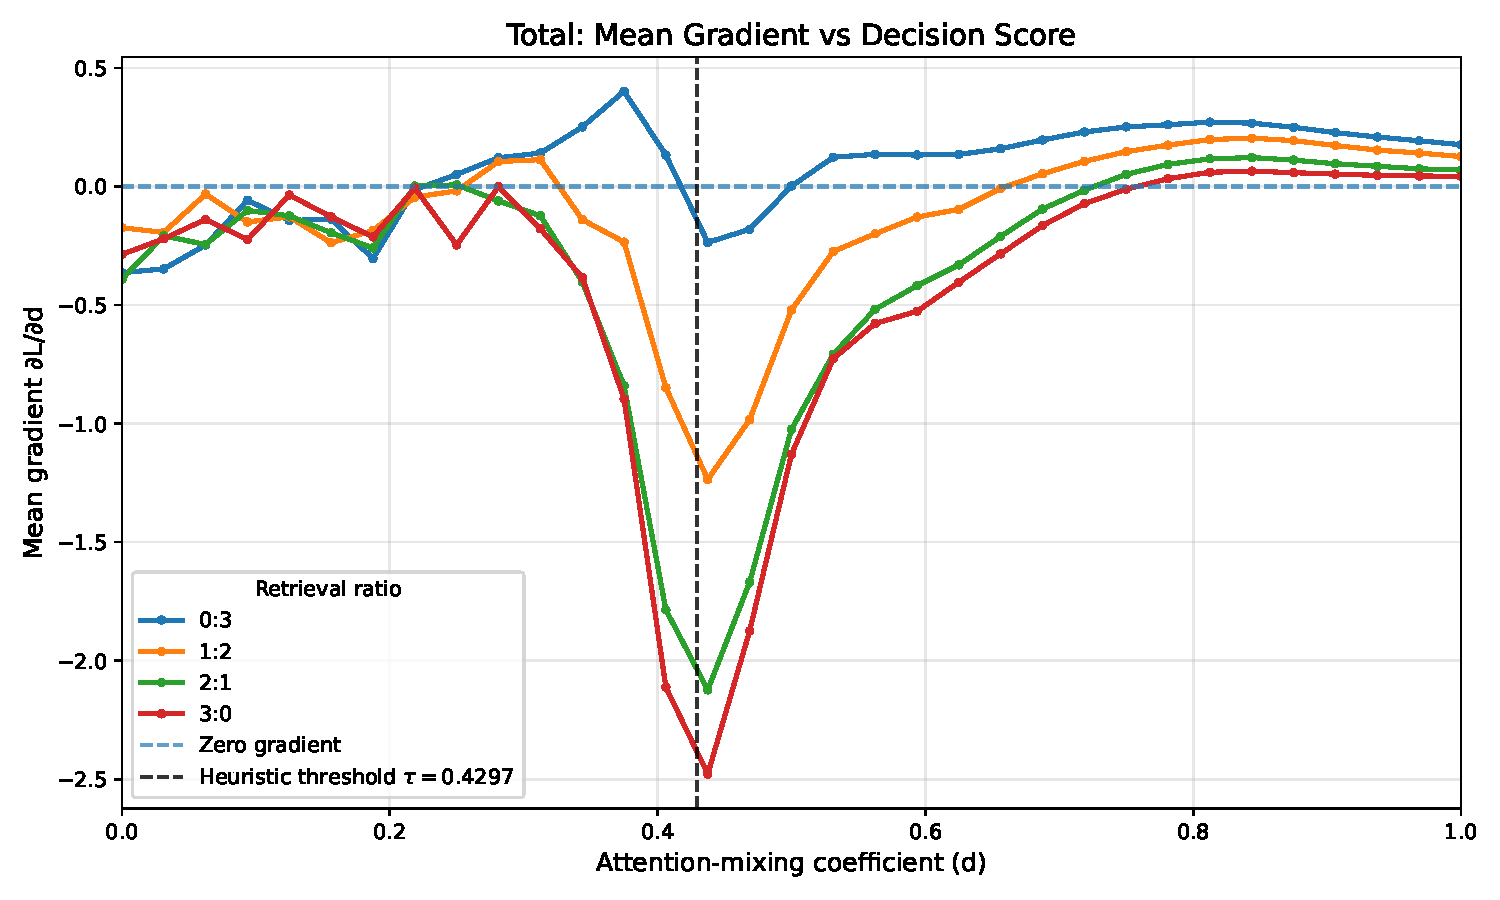
\includegraphics[width=.86\linewidth]{graphics/h2-gradient.pdf}
\caption{H2: gradient mất mát trung bình theo \(d\). Vạch đứng chỉ ngưỡng vận hành \(\tau\) để tham chiếu. Nguồn: notebook H2, ô vẽ đường gradient.}
\label{fig:h2}
\end{figure}
\begin{figure}[htbp]\centering
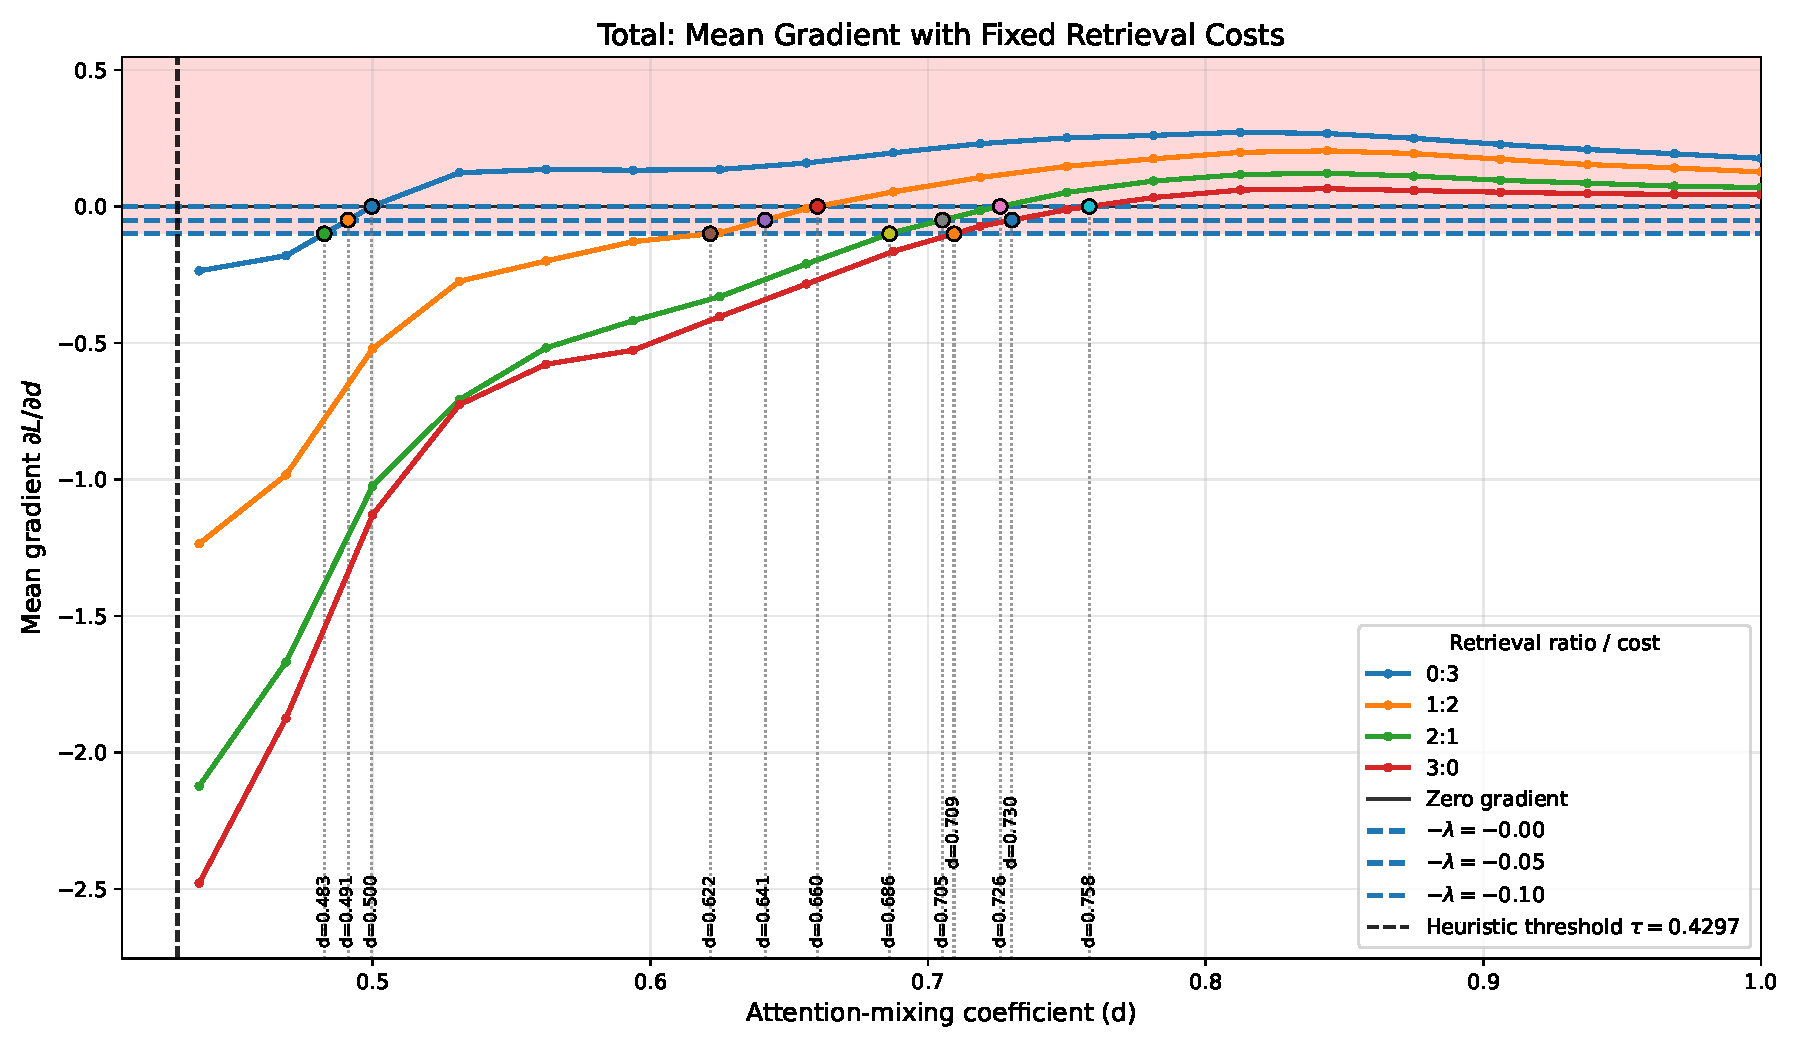
\includegraphics[width=\linewidth]{graphics/h2-cost.pdf}
\caption{H2: đối chiếu gradient với các mức \(-\lambda\). Nguồn: ô phân tích chi phí trong cùng notebook.}
\label{fig:h2cost}
\end{figure}
\clearpage
\subsection{Chất lượng hỏi đáp và tải truy hồi}
\begin{table}[htbp]\centering\small
\caption{Đối chứng địa phương, 500 mẫu mỗi bộ. ART dùng ngưỡng 0.4297. Chỉ số theo phần trăm.}
\label{tab:local}
\begin{tabular}{@{}llrrrl@{}}
\toprule
Bộ dữ liệu & Hệ thống & Acc & F1 & EM & ID \\
\midrule
MuSiQue & No-RAG & 0.80 & 5.61 & 0.60 & M05 \\
 & Vanilla RAG & 6.20 & 10.25 & 4.80 & M06 \\
 & ART & 25.80 & 31.17 & 21.60 & M12 \\
HotpotQA & No-RAG & 14.00 & 20.19 & 14.20 & M03 \\
 & Vanilla RAG & 33.20 & 39.61 & 30.20 & M04 \\
 & ART & 42.20 & 48.24 & 37.20 & M08 \\
2WikiMultiHopQA & No-RAG & 24.80 & 27.58 & 24.40 & M01 \\
 & Vanilla RAG & 34.80 & 37.81 & 32.20 & M02 \\
 & ART & 48.20 & 46.30 & 37.00 & M07 \\
\bottomrule
\end{tabular}
\end{table}

\Cref{tab:local} cho thấy ART ở ngưỡng mặc định cải thiện cả ba chỉ số trên cả ba bộ. So với Vanilla RAG, F1 tăng \(20.92\), \(8.63\), \(8.49\) điểm phần trăm theo thứ tự MuSiQue, HotpotQA, 2WikiMultiHopQA. So với No-RAG, mức tăng tương ứng là \(25.56\), \(28.05\), \(18.72\). Đây là kết quả của hệ thống hoàn chỉnh chứa cả quá trình tinh chỉnh và chính sách truy hồi.
\Cref{tab:sweep,fig:tradeoff} tóm tắt các cấu hình có ngưỡng xác định.
\begin{table}[htbp]\centering\small
\caption{Quét ngưỡng ART. TB là truy vấn/mẫu, Có (\%) là tỷ lệ mẫu có truy vấn và Tổng là số truy vấn ghi nhận.}
\label{tab:sweep}
\begin{tabular}{@{}lrrrrrrr@{}}
\toprule
Bộ dữ liệu & $\tau$ & Acc & F1 & EM & TB & Có (\%) & Tổng \\
\midrule
MuSiQue & 0.4297 & 25.80 & 31.17 & 21.60 & 4.792 & 100.0 & 2396 \\
 & 0.50 & 24.00 & 30.27 & 20.80 & 3.594 & 100.0 & 1797 \\
 & 0.60 & 26.00 & 32.08 & 22.80 & 2.588 & 100.0 & 1294 \\
 & 0.70 & 22.60 & 29.21 & 19.80 & 2.126 & 99.2 & 1063 \\
HotpotQA & 0.4297 & 42.20 & 48.24 & 37.20 & 4.070 & 100.0 & 2035 \\
 & 0.50 & 43.80 & 49.68 & 39.20 & 3.166 & 99.8 & 1583 \\
 & 0.60 & 40.00 & 46.87 & 36.40 & 2.278 & 99.2 & 1139 \\
2WikiMultiHopQA & 0.4297 & 48.20 & 46.30 & 37.00 & 4.012 & 100.0 & 2006 \\
 & 0.50 & 46.40 & 44.75 & 35.60 & 2.930 & 100.0 & 1465 \\
 & 0.60 & 44.40 & 44.34 & 36.00 & 2.126 & 99.4 & 1063 \\
\bottomrule
\end{tabular}
\end{table}


Retrieval count là số truy vấn ghi nhận trên mỗi mẫu hoàn tất, tính cả truy vấn lặp. Trên cả ba benchmark, số lượt trung bình giảm khi tăng \(\tau\) trong các cấu hình đã khảo sát. F1 giảm liên tiếp trên 2WikiMultiHopQA, tăng rồi giảm trên HotpotQA, và giảm, phục hồi rồi giảm lại trên MuSiQue. Chẳng hạn, MuSiQue ở ngưỡng \(0.60\) có 2.588 truy vấn trung bình và F1 32.08, so với 4.792 truy vấn và F1 31.17 ở cấu hình chuẩn. Ít truy vấn hơn có thể đi kèm F1 cao hơn hoặc thấp hơn tùy cấu hình. Số truy vấn phản ánh mức sử dụng truy hồi; các lượt chạy này không đo latency, FLOPs hay tổng compute.

\begin{figure}[htbp]\centering
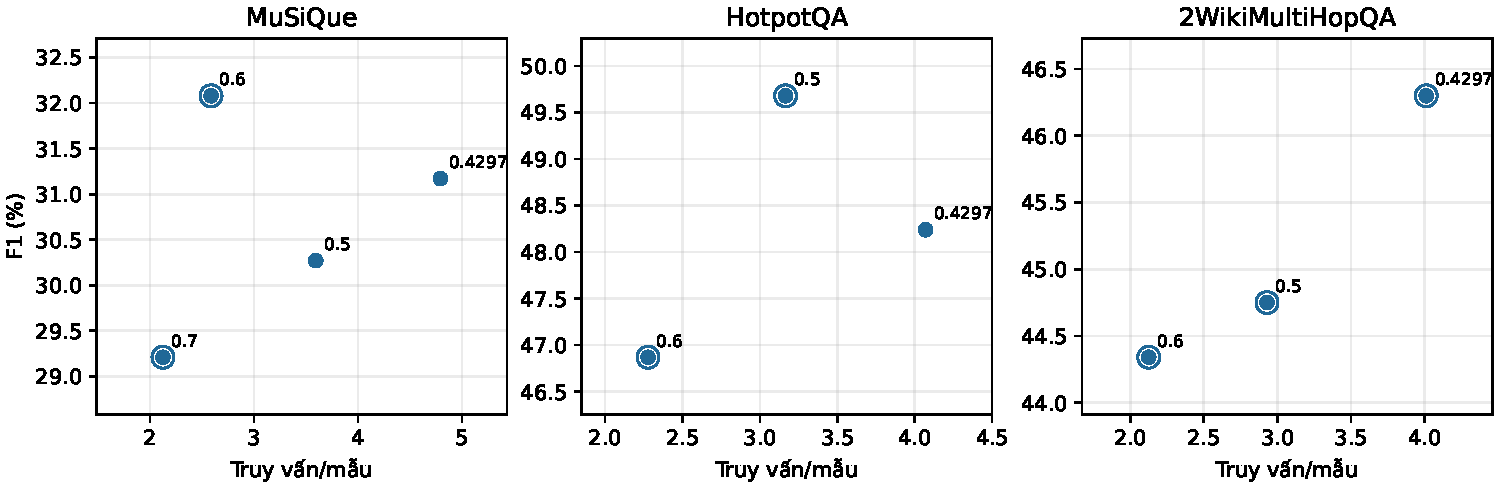
\includegraphics[width=\linewidth]{graphics/tradeoff.pdf}
\caption{F1 và số truy vấn trung bình trên các cấu hình có ngưỡng xác định. Các nhãn điểm là ngưỡng quyết định.}
\label{fig:tradeoff}
\end{figure}
\clearpage
\section{Thảo luận}
\subsection{Ví dụ đối sánh trên MuSiQue}
Ví dụ MuSiQue ID 348 ở \cref{fig:baseline-case} có EM bằng 0 với No-RAG và Vanilla RAG, và bằng 1 với ART. Đáp án của ART là \emph{Snapper Foster}. Phụ lục~\ref{app:examples} lưu nguyên văn các đầu ra và đoạn truy hồi.

Ở lượt đầu, đoạn \emph{Michael Knight (Knight Rider)} xác định David Hasselhoff là diễn viên. Lượt sau đưa tên David Hasselhoff vào truy vấn và trả về đoạn \emph{Snapper Foster}, nơi ghi rõ ông từng đóng vai này. Vanilla RAG có bằng chứng cho quan hệ đầu tiên trong năm đoạn đã lưu, nhưng thiếu đoạn xác nhận vai diễn. Chuỗi quan sát minh họa cách truy vấn được cập nhật theo thông tin đã tìm thấy. So sánh hệ thống này chưa cô lập ảnh hưởng của retrieval timing.

\subsection{So sánh cơ chế}
Các phương pháp IRCoT, Self-RAG và R-Search\cite{ircot,selfrag,rsearch} tiếp cận bài toán truy hồi thích nghi theo những cơ chế khác nhau. IRCoT kết hợp truy hồi với các bước suy luận trung gian; Self-RAG sử dụng các reflection tokens được học từ tín hiệu giám sát để điều khiển truy hồi; trong khi R-Search tối ưu quá trình tìm kiếm thông qua tín hiệu phần thưởng.

Khác với các phương pháp trên, ART kết hợp LM Loss với Retrieval Regularization trong cùng mục tiêu huấn luyện. Thông qua Attention Mixing, tín hiệu gradient từ quá trình dự đoán token có thể tác động gián tiếp đến Decision Head, giúp mô hình học cách điều chỉnh quyết định truy hồi mà không cần nhãn trực tiếp cho từng thời điểm truy hồi hoặc tối ưu chính sách bằng Reinforcement Learning. Tuy nhiên, ART vẫn sử dụng dữ liệu đích do teacher model tạo ra và quá trình Collect–Replay để tổ chức huấn luyện.

Kết quả thực nghiệm cho thấy hiệu quả của hệ thống ART hoàn chỉnh trên các bộ dữ liệu được khảo sát. Tuy nhiên, do ART sử dụng checkpoint đã fine-tune, trong khi các baseline sử dụng checkpoint gốc, kết quả hiện tại chưa tách biệt được đóng góp riêng của cơ chế lựa chọn thời điểm truy hồi. Để đánh giá riêng tác động này, cần thực hiện thêm các thí nghiệm ablation với checkpoint và điều kiện đánh giá tương thích.
